\section{Monday 09/16/2024}
\subsection{Review}
\subsubsection{Problem formulation for multiple constraints}

\begin{equation}
  \begin{aligned}
    \min f(x) \\
    s.t. g_1(x) \leq 0 \\
    g_2(x) \leq 0
  \end{aligned}
\end{equation}
The difference between a function and a tiny step of size $\delta$ in direction $d$ can be approximated as the inner product between the gradient of the function and the step $\delta d$
\begin{equation}
  \begin{aligned}
    f(x + \delta d) - f(x) \approx \langle \nabla f(x),  \delta d \rangle \\
    g_1(x + \delta d) - g_1(x) \approx \langle \nabla g_1(x),  \delta d \rangle \\
    g_2(x + \delta d) - g_2(x) \approx \langle \nabla g_2(x),  \delta d \rangle \\
    g_1(x) = 0, g_2(x) = 0
  \end{aligned}
\end{equation}
In order for the constraints set in the general minimization problem to be met, the inner product between the gradient of the constraint and the step should be non-positive. We can define the "walkable" region as the intersection of the halfspaces created by the negative gradients of the objective function and any constraints. For a solution to be optimal, this intersection must be empty.
\subsubsection{Optimality}
A minimal solution is reached when
\begin{equation}
  \nabla f(x^*) + \gamma_1 \nabla g_1(x^*) + \gamma_2 \nabla g_2(x^*)  = 0
\end{equation}
where $\gamma_1 \geq 0, \gamma_2 \geq 0$
\\ \\
This is a non-negative linear combination of the gradient vectors. The set of all non-negative linear combinations of two vectors $u$ and $v$ is a cone with edges on $u$ and $v$. This cone can be parametrized by a single scalar $w$ using the following
\begin{equation}
  \begin{aligned}
    w(r_1 u + r_2 v) = y \\
    r_1+ r_2 = 1 \\
    r_1 \geq 0, r_2 \geq 0, w \geq 0
  \end{aligned}
\end{equation}
Using that logic to explain the equation $\nabla f(x^*) + \gamma_1 \nabla g_1(x^*) + \gamma_2 \nabla g_2(x^*)  = 0$, there is a vector $\nabla f$ that is opposite of any linear combination of the constraints.

\begin{figure}[htbp]
  \centerline{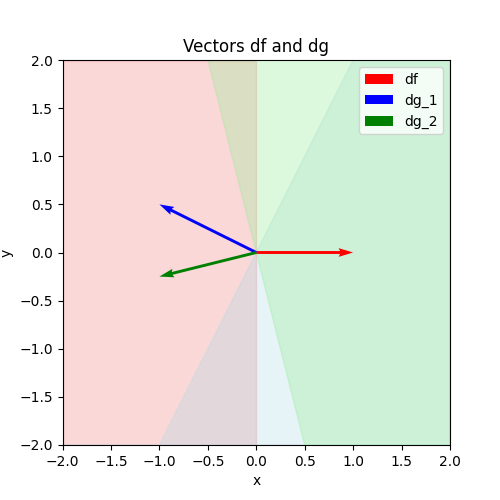
\includegraphics[width=0.75\textwidth]{images/empty_walkable_region.png}}
  \caption{Image of an empty walkable region since $\nabla f$ is opposite of $\nabla g$}
  \label{fig:empty_walkable_region}
\end{figure}

\subsection{Active constraints}
In an optimization problem such as the bowl, it is possible that there is only one active constraint, to the problem. Therefore, although $g_1$ and $g_2$ are defined, only one is relevant to the optimization problem.
\begin{equation}
  \nabla f(x^*) + \gamma_1 \nabla g_1(x^*) + \gamma_2 \nabla g_2(x^*)  = 0
\end{equation}
where $\gamma_1 \geq 0, \gamma_2 \geq 0$ when there is only one active constraint, is equivalent to
\begin{equation}
  \nabla f(x^*) + \gamma_1 \nabla g_1(x^*)  = 0
\end{equation}
where $\gamma_1 \geq 0 $
\\ \\
Can we alter the first rule to incorporate this new information of potentially inactive constraints? Adding binary variables.

\section{Wednesday 09/18/2024}
\subsection{Multiple Constraints}
\subsubsection{Inactive constraints}
Could have the case where two constraints are defined but only one is active optimal solution

\begin{equation}
  \begin{aligned}
    \min f(x) \\
    s.t. g_1(x) \leq 0 \\
    g_2(x) \leq 0
  \end{aligned}
\end{equation}

\begin{equation}
  \text{Inactive Case: }
  \begin{aligned}
    \nabla f(x^*) + \gamma_1 \nabla g_1(x^*)  = 0 \\
    g_1(x^*) = 0, \gamma_1 \geq 0
  \end{aligned}
\end{equation}

\begin{equation}
  \text{Active Case: }
  \begin{aligned}
    \nabla f(x^*) + \gamma_1 \nabla g_1(x^*) + \gamma_2 \nabla g_2(x^*)  = 0 \\
    g_1(x^*) = 0, g_2(x^*) = 0, \gamma_1 \geq 0, \gamma_2 \geq 0
  \end{aligned}
\end{equation}

Both cases can be captured when $\nabla g_2 < 0, \gamma_2 = 0$ or  $\nabla g_2 = 0, \gamma_2 \geq 0$. Those two scenarios are captured by the equation 
\begin{equation}
  \gamma_2 g_2(x^*) = 0
\end{equation}
\subsubsection{Karush-Kahn-Tucker Conditions}
\begin{equation}
  \begin{aligned}
    \min f(x) \\
    s.t. g_1(x) \leq 0 \\
    g_2(x) \leq 0
  \end{aligned}
\end{equation}
is minimized when 
\begin{equation}
  \text{Final System: }
  \begin{aligned}
    \nabla f(x^*) + \gamma_1 \nabla g_1(x^*) + \gamma_2 \nabla g_2(x^*)  = 0 \\
    g_1(x^*) \leq 0, g_2(x^*) \leq 0, \gamma_1 \geq 0, \gamma_2 \geq 0, \\
    \gamma_1 g_1(x^*)=0, \gamma_2 g_2(x^*) = 0
  \end{aligned}
\end{equation}
\subsection{Adding an equality constraint}
Can split an equality constraint into two inequalities.
\begin{equation}
  \begin{aligned}
    \min f(x) \\
    h(x) = 0
  \end{aligned}
  \text{ or }
  \begin{aligned}
    \min f(x) \\
    h(x) \leq 0, h(x) \geq 0
  \end{aligned}
\end{equation}
is satisfied when
\begin{equation}
  \begin{aligned}
    \nabla f(x^*) + \gamma_1 \nabla h(x^*) - \gamma_2 \nabla h(x^*)  = 0 \\
    h(x^*) \leq 0, h(x^*) \geq 0, \gamma_1 \geq 0, \gamma_2 \geq 0, \\
    \gamma_1 h(x^*)=0, \gamma_2 h(x^*) = 0
  \end{aligned}
\end{equation}
Which can be simplified to 
\begin{equation}
  \begin{aligned}
    \nabla f(x^*)+ \hat{\gamma} \nabla h(x^*)  = 0 \\
    h(x^*) =0
  \end{aligned}
\end{equation}
\subsection{KKT Conditions General Case}
Under a constraint qualification, a local optimal solution satisfies the conditions
\begin{equation}
  \begin{aligned}
    \nabla f(x^*) + [\nabla h(x^*)]^T \Theta + [\nabla g(x^*)]^T \Gamma = 0, \\
    [g(x^*)]^T\Gamma = 0, \\
    \Gamma \geq 0, \\
    h(x^*) = 0, g(x^*) \leq 0
  \end{aligned}
\end{equation}
\subsubsection{KKT Solutions example}
\begin{equation}
  \begin{aligned}
    \min_{x_1,x_2} x_1^2 + x_2^2 \\
    s.t. x_1 + 2x_2 \leq -1 \\
    x_1+x_2 = -3 \\
    x_1 \geq 0
  \end{aligned}
\end{equation}
THe KKT solutions

\begin{align}
  \begin{bmatrix}
     2x_1 \\
     2x_2
  \end{bmatrix}
  +
  \gamma_1
  \begin{bmatrix}
    1 \\
    2
  \end{bmatrix}
  +
  \gamma_2
  \begin{bmatrix}
    1 \\
    1
  \end{bmatrix}
  -
  \gamma_3
  \begin{bmatrix}
    1 \\
    0
  \end{bmatrix}
  = 0
\end{align}

\begin{equation}
  \begin{aligned}
    \gamma_1 \geq 0, \gamma_3 \geq 0, x_1 + 2x_2 \leq -1, x_1+x_2 = -3
  \end{aligned}
\end{equation}